\documentclass[10pt, a4paper]{article}
\usepackage[spanish]{babel} % espanol.
%Lo pongo en english para que me compile :S.

\usepackage[utf8]{inputenc}
\usepackage{enumerate} % enumerados
\usepackage{graphicx}
\usepackage{longtable}
\usepackage{multicol}
\graphicspath{ {img/} }
\usepackage[paper=a4paper, left=1.5cm, right=1.5cm, bottom=1.5cm, top=3.5cm]{geometry}
\usepackage{indentfirst}
\usepackage{fancyhdr}
\usepackage{color}
\usepackage[colorlinks=true, linkcolor=black]{hyperref}
\usepackage{a4wide}
\usepackage{tikz}
\usepackage{epsf}
\usepackage{caratula}

\begin{document}


\begin{figure}[ptb]

\includegraphics[scale=0.30]{logo.jpg}\hspace{6cm}

\includegraphics[scale=0.90]{logo_dc.jpg}
\end{figure}

%Datos de la caratula
\materia{Redes Neuronales}
\titulo{Trabajo pr\'actico 1}
\subtitulo{Parser}
\hspace{6cm}
\integrante{Negri, Franco}{893/13}{franconegri2004@hotmail.com}
\integrante{?, ?}{?/?}{?@?.com}
\palabrasClave{TP}
  % Reconocimiento caras. PCA. Power Method. Deflation. Autovalores. Autovectores. Matriz
  % semi definida positiva.

\resumen{Entrenamiento de Redes Neuronales}

\parskip=5pt % 10pt es el tamaño de fuente

% Pongo en 0 la distancia extra entre ítemes.
\let\olditemize\itemize
\def\itemize{\olditemize\itemsep=0pt}

% Acomodo fancyhdr <- Creo que es el encabezado de pagina
\pagestyle{fancy}
\thispagestyle{fancy}
\addtolength{\headheight}{1pt}
%\lhead{Acosta, Negri}
%\rhead{1$^{do}$ Cuatrimestre 2016}
\cfoot{\thepage}
\renewcommand{\footrulewidth}{0.4pt}




%Pagina de titulo e indice
\thispagestyle{empty}

\maketitle



\tableofcontents
\section{Introduccion}
En este trabajo, nos disponesmos a utlizar diferentes tecnicas de aprendisaje no supervisado para clasificar textos con ciertas caracteristicas. Los mismos consisten en descripciones de diversas companías y nuestro objetivo será lograr clasificar cada una en una categoria correspondiente.

\section{Desarrollo}
\subsection{PCA}
EL primer modelo utilizado para intentar clasificar los datos será el de Analisis de Componentes Principales. Para ello utilizamremos dos algoritmos basados en aprendisaje Hebbiano y reduciremos las instancias de entrenamiento a 3 dimenciones. Lo que esperamos observar es que aquellas instancias que pertenecen a una misma clase de empresa se encuentran cercas unas de otras, pudiendo observar \"nuves\" de puntos bien definidas.

\subsubsection{Implementación}

En particular los algoritmos utilizados serán los de $Oja$ y $Sanger$. Teniendo una complegidad computacional identica y siendo los algoritmos muy similares, lo distintivo entre estos dos metodos es que $Sanger$ ordenará las componentes prinsipales de mayor a menor de acuerdo a sus autovalores mientras que $Oja$ no.

El pseodocodigo utilizado para aprendisaje del algoritmo $Oja$ será:

\begin{algorithm}
\begin{algorithmic}[1]\parskip=1mm
 \caption{ Algoritmo De Oja}
 \STATE{Para toda instancia de entrenamiento, x}
 \STATE{\quad $y = x.W$}
 \STATE{\quad $\tilde x = y.W^T$}
 \STATE{\quad $\Delta W = learning\_rate ((x - \tilde x)^T . y$}
\end{algorithmic}
\end{algorithm}

Mientras que el de $Sanger$

\begin{algorithm}
\begin{algorithmic}[1]\parskip=1mm
 \caption{ Algoritmo De Sanger}
 \STATE{U = Matriz Triangular Superior Con 1s}
 \STATE{Para toda instancia de entrenamiento, x}
 \STATE{\quad $y = x.W$}
 \STATE{\quad $\tilde x = W(y^T.U)$}
 \STATE{\quad $\Delta W = learning\_rate ((x^T - \tilde x) . y$}
\end{algorithmic}
\end{algorithm}

Utilizando el paquete numpy de python es posible traducir este codigo de manera casi exacta y de esa manera aprovechar las optimizaciones matriciales que se realizan sobre los datos.

\subsubsection{Experimentación}

Para la experimentación entrenamos la red con parte del set de datos que nos fue entregado

\begin{figure}[h!]
\centering
\begin{subfigure}{.5\textwidth}
  \centering
  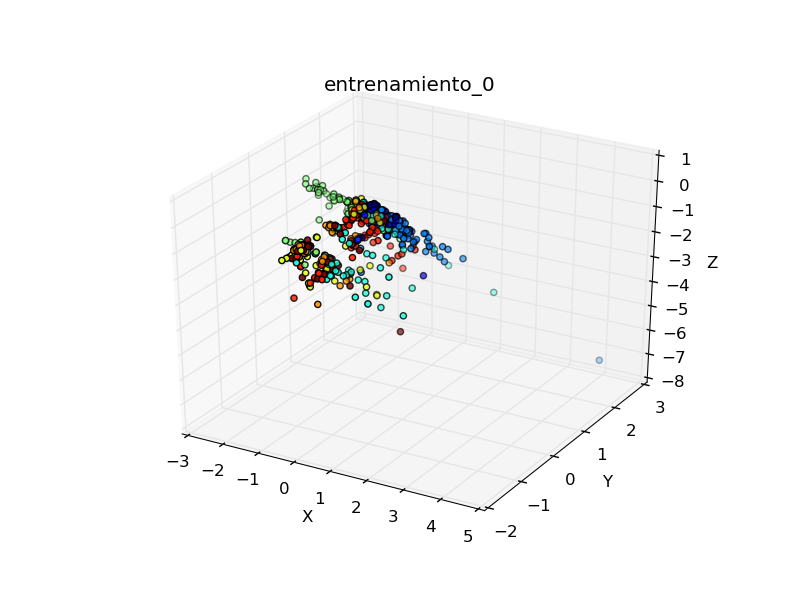
\includegraphics[width=.4\linewidth]{convergencia_oja/entrenamiento_0.png}
  \caption{A subfigure}
  \label{fig:sub1}
\end{subfigure}%
\begin{subfigure}{.5\textwidth}
  \centering
  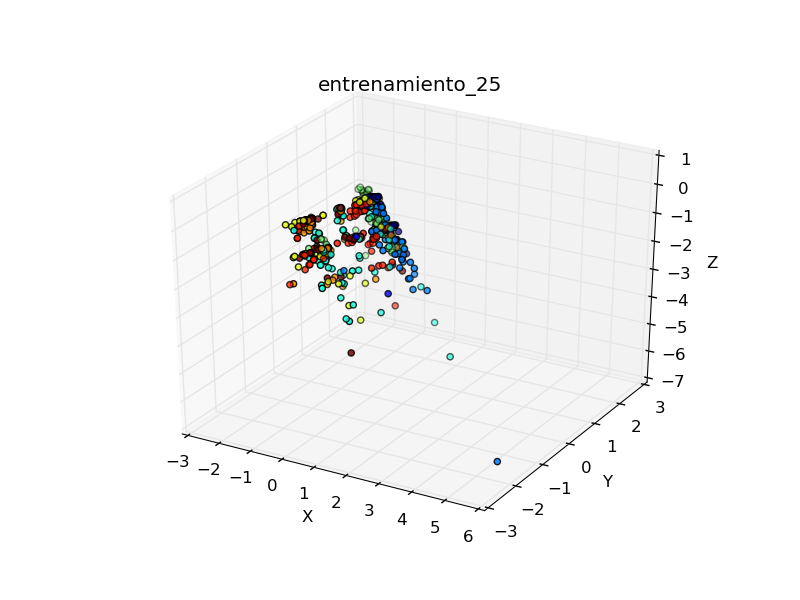
\includegraphics[width=.4\linewidth]{convergencia_oja/entrenamiento_25.png}
  \caption{A subfigure}
  \label{fig:sub2}
\end{subfigure}
\caption{A figure with two subfigures}
\label{fig:test}
\end{figure}

\begin{figure}[h!]
\centering
\begin{subfigure}{.5\textwidth}
  \centering
  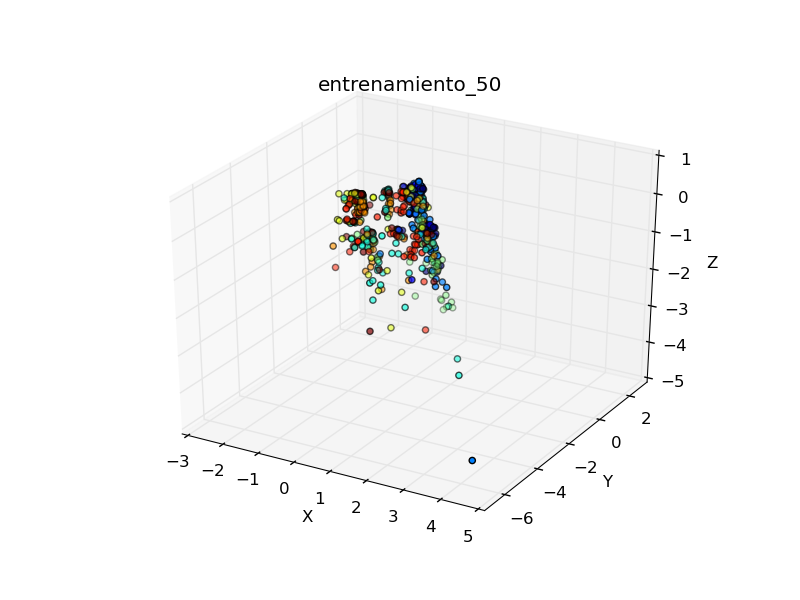
\includegraphics[width=.4\linewidth]{convergencia_oja/entrenamiento_50.png}
  \caption{A subfigure}
  \label{fig:sub1}
\end{subfigure}%
\begin{subfigure}{.5\textwidth}
  \centering
  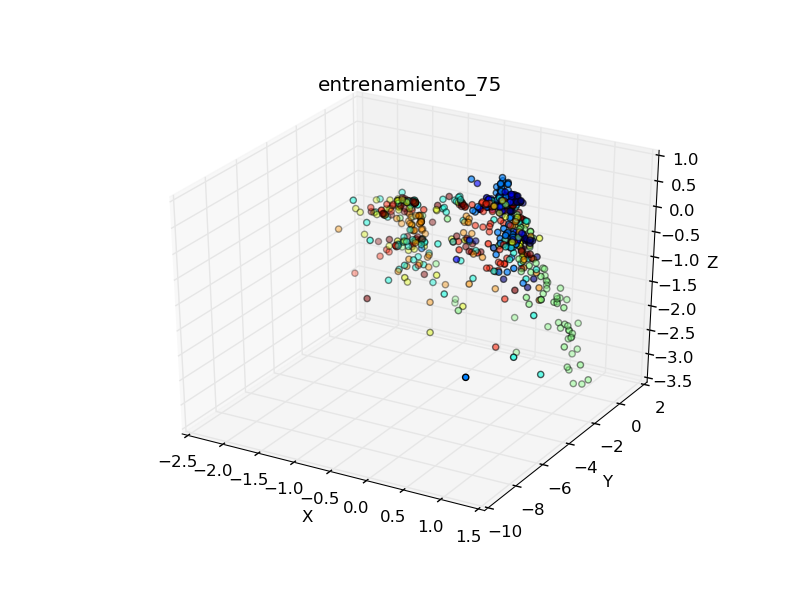
\includegraphics[width=.4\linewidth]{convergencia_oja/entrenamiento_75.png}
  \caption{A subfigure}
  \label{fig:sub2}
\end{subfigure}
\caption{A figure with two subfigures}
\label{fig:test}
\end{figure}

\begin{figure}[h!]
	\centering
	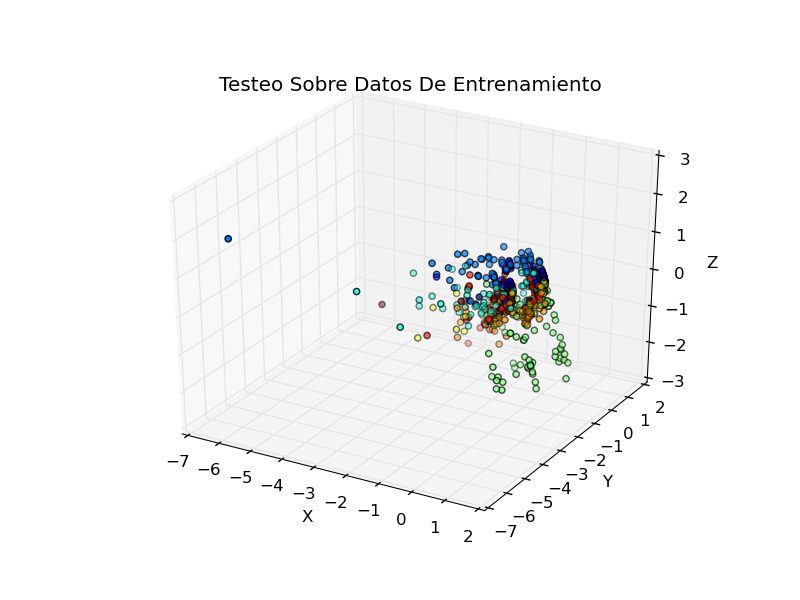
\includegraphics[width=.5\linewidth]{convergencia_oja/entrenamiento_100.png}
	\captionof{figure}{A figure}
	\label{fig:test1}
	\centering
\end{figure}

\pagebreak
Sanger

\begin{figure}[h!]
\centering
\begin{subfigure}{.5\textwidth}
  \centering
  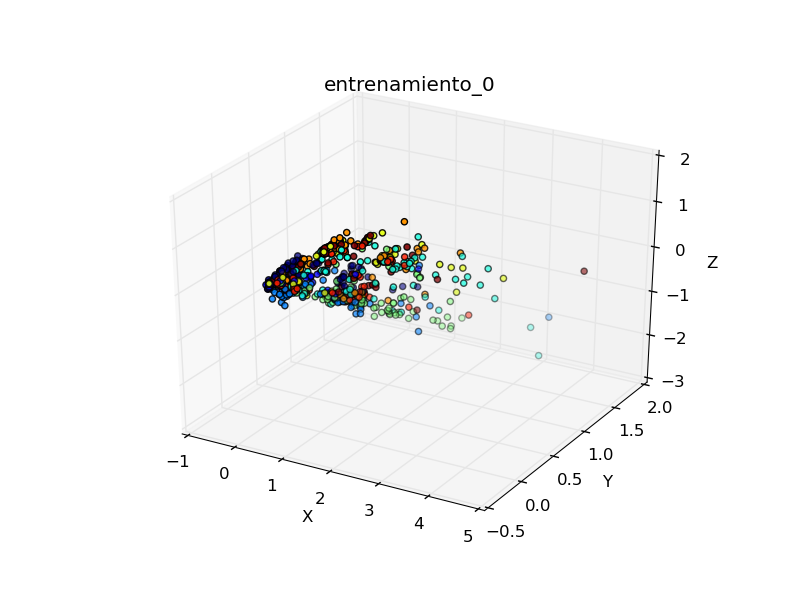
\includegraphics[width=.4\linewidth]{convergencia_sanger/entrenamiento_0.png}
  \caption{A subfigure}
  \label{fig:sub1}
\end{subfigure}%
\begin{subfigure}{.5\textwidth}
  \centering
  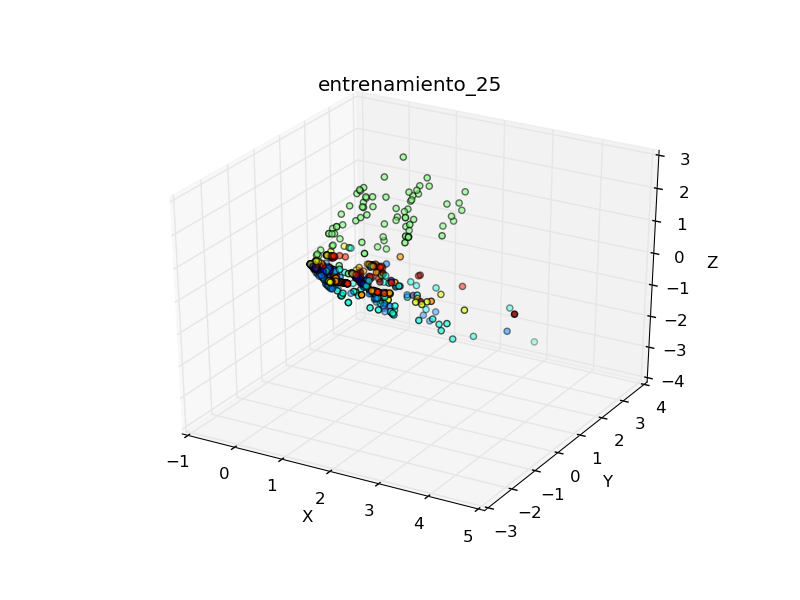
\includegraphics[width=.4\linewidth]{convergencia_sanger/entrenamiento_25.png}
  \caption{A subfigure}
  \label{fig:sub2}
\end{subfigure}
\caption{A figure with two subfigures}
\label{fig:test}
\end{figure}

\begin{figure}[h!]
\centering
\begin{subfigure}{.5\textwidth}
  \centering
  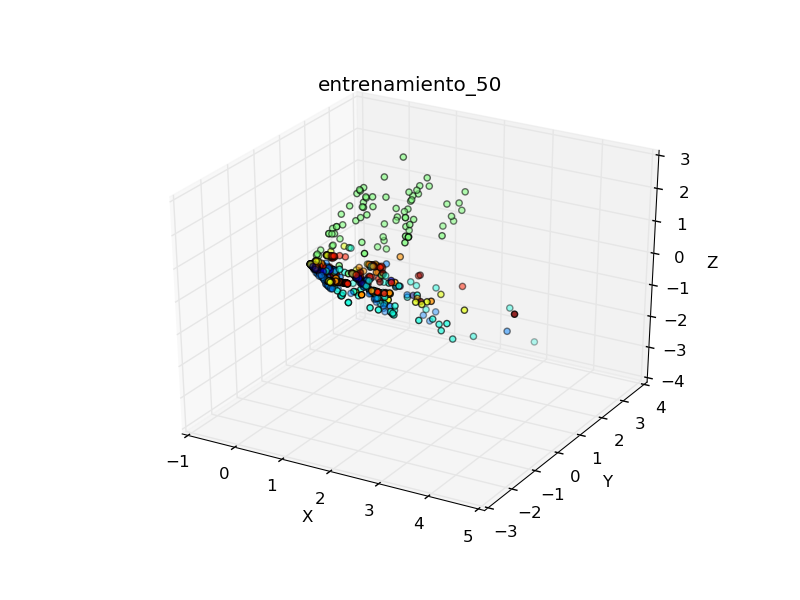
\includegraphics[width=.4\linewidth]{convergencia_sanger/entrenamiento_50.png}
  \caption{A subfigure}
  \label{fig:sub1}
\end{subfigure}%
\begin{subfigure}{.5\textwidth}
  \centering
  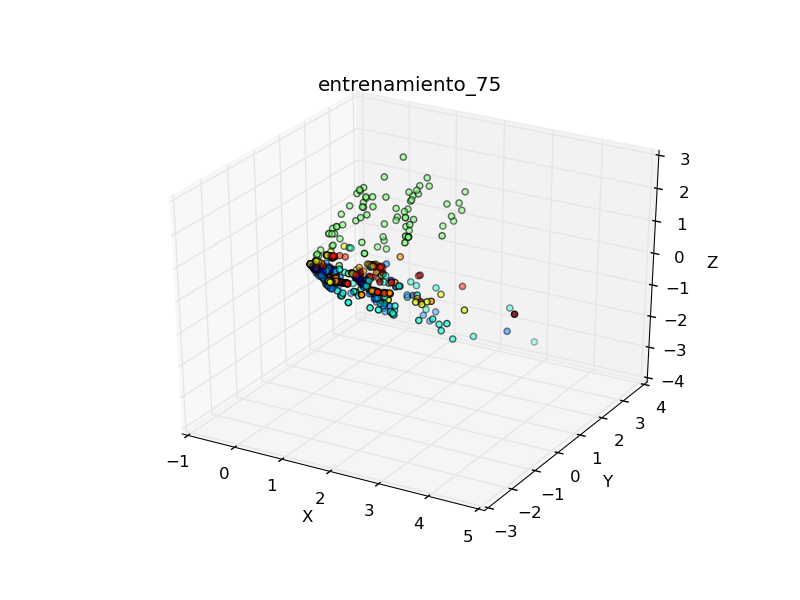
\includegraphics[width=.4\linewidth]{convergencia_sanger/entrenamiento_75.png}
  \caption{A subfigure}
  \label{fig:sub2}
\end{subfigure}
\caption{A figure with two subfigures}
\label{fig:test}
\end{figure}

\begin{figure}[h!]
	\centering
	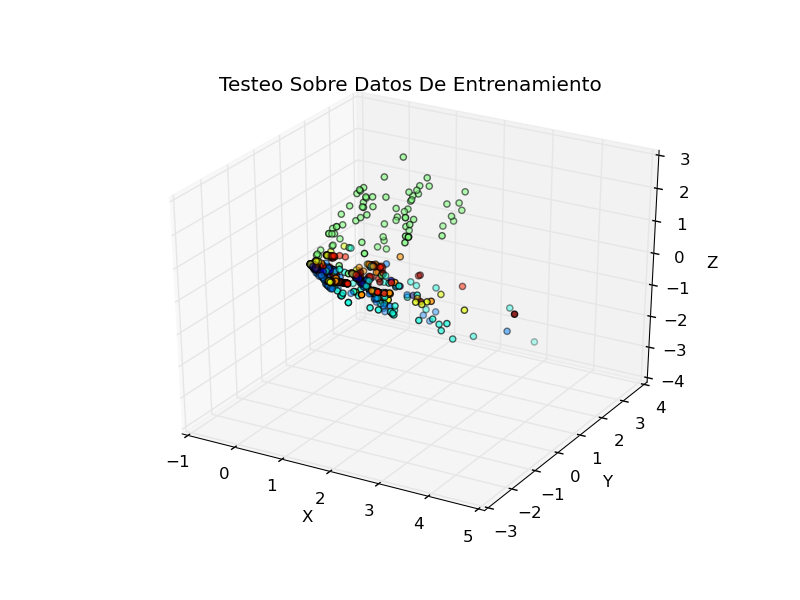
\includegraphics[width=.5\linewidth]{convergencia_sanger/entrenamiento_100.png}
	\captionof{figure}{A figure}
	\label{fig:test1}
	\centering
\end{figure}

%Neural Networks Haykin
% In Chatterjee et al. (1998), the convergence properties of the GHA algorithm
% described in Eq. (8.91) are investigated. The analysis presented therein shows that
% increasing  leads to faster convergence and larger asymptotic mean-square error, which
% is intuitively satisfying. In that paper, the tradeoff between the accuracy of computation
% and speed of learning is made explicit.



\subsection{Mapeo de Características}

En este apartado construiremos un modelo de mapeo de caracteristicas auto-organizado con la intención de clasificar los documentos en un arreglo de dos dimenciones. Para ello utilizaremos el algoritmo de Kohonen sobre los datos de entrenamiento y una vez que la red haya convergido, graficaremos los las respuestas obtenidas en el plano.

Convergencia Kohonen

\begin{figure}[h!]
\centering
\begin{minipage}{.15\textwidth}
  \centering
  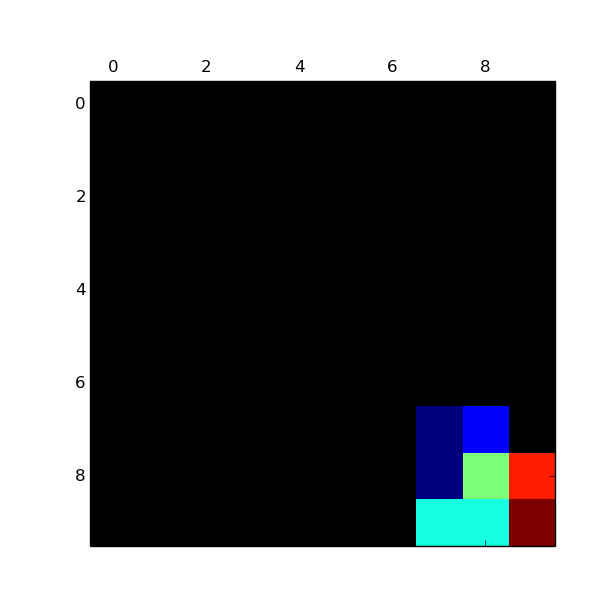
\includegraphics[width=.9\linewidth]{convergencia_kohonen/entrenamiento_0.png}
  \captionof{figure}{0\%}
  \label{fig:test1}
\end{minipage}%
\begin{minipage}{.15\textwidth}
  \centering
  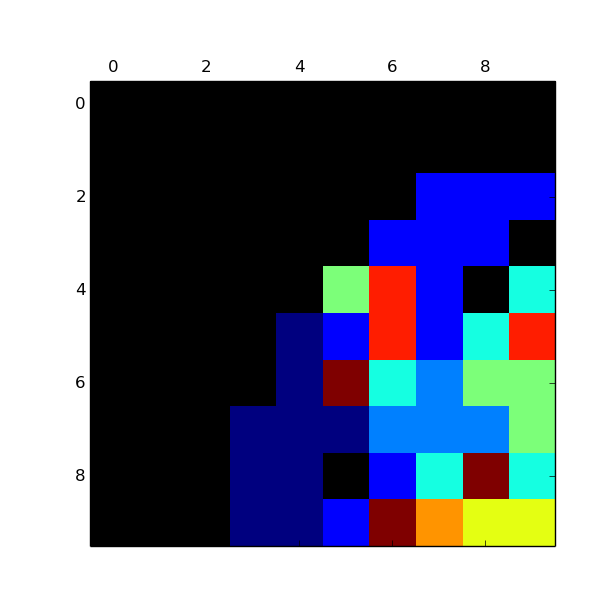
\includegraphics[width=.9\linewidth]{convergencia_kohonen/entrenamiento_25.png}
  \captionof{figure}{25\%}
  \label{fig:test2}
\end{minipage}
\begin{minipage}{.15\textwidth}
  \centering
  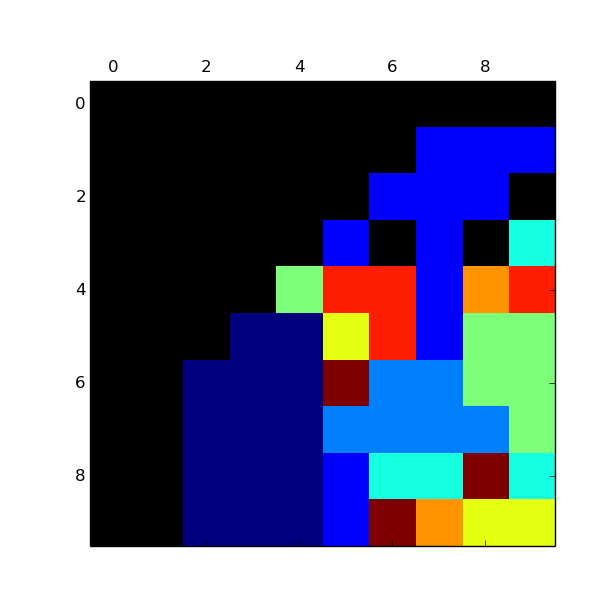
\includegraphics[width=.9\linewidth]{convergencia_kohonen/entrenamiento_50.png}
  \captionof{figure}{50\%}
  \label{fig:test2}
\end{minipage}
\begin{minipage}{.15\textwidth}
  \centering
  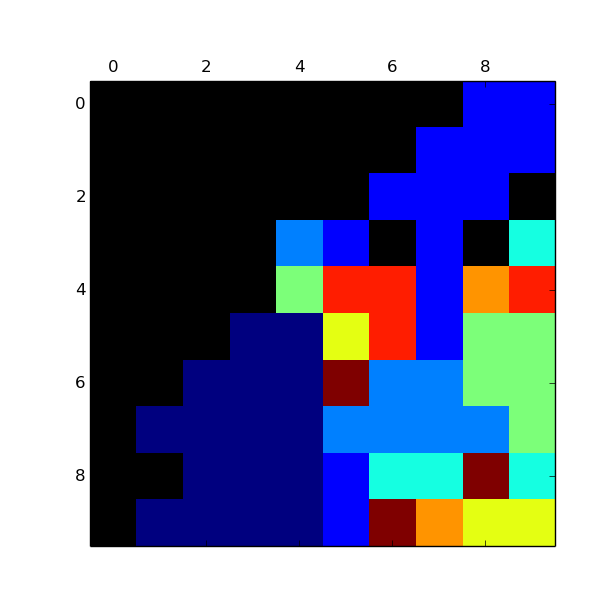
\includegraphics[width=.9\linewidth]{convergencia_kohonen/entrenamiento_75.png}
  \captionof{figure}{75\%}
  \label{fig:test2}
\end{minipage}
\begin{minipage}{.15\textwidth}
  \centering
  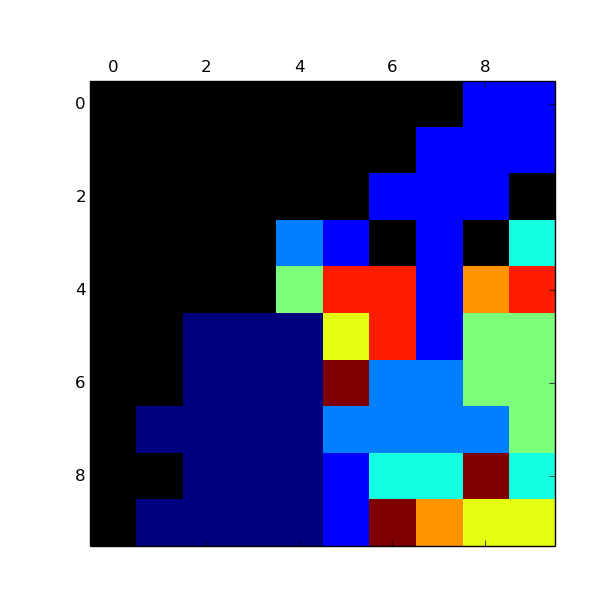
\includegraphics[width=.9\linewidth]{convergencia_kohonen/entrenamiento_100.png}
  \captionof{figure}{100\%}
  \label{fig:test2}
\end{minipage}
\end{figure}
\section{Concluciones}
PCA: Podemos observar que a medida que aumentamos la cantidad de épocas los datos tienden a esparcirse mas, y esto claramente es debido a que el algoritmo lo que hace es maximizar la varianza. Es decir, en otros términos lo que trata de hacer es lo siguiente:
Tenemos 3 ejes en los cuales podemos representar nuestros datos. Inicialmente todos los puntos estan muy pegados los unos a los otros. Es como si tuviesemos una cámara fotográfica y sacaramos una foto en cierto ángulo viendo todos los puntos unos encima de los otros. A medida que aumentan las iteraciones lo que el algoritmo trata de hacer es cambiar el ángulo de nuestra cámara para poder ver a cada uno de los puntos de manera mas separada posible de sus aledaños para poder en una misma captura, verlos a todos sin que se encimen. Por eso cuando el algoritmo converge, podemos observar a los puntos esparcidos en el espacio, obteniendo la mayor cantidad de información (ya que por ejemplo, si estan todos pegoteados, no tengo forma de separarlos mediante planos por ejemplo para clasificacion, ahora bien si los trato de representar en un sistema de componentes principales quizá estos se separen lo suficiente que me permitan separarlos).

SOM: Podemos ver que claramente en un 25\% de entrenamiento, el algoritmo ya logro su ordenamiento. Lo que resta (es decir las iteraciones restantes) son simplemente para la convergencia del mismo. Esto es fundamentado en el libro de Haykin donde se establece que alrededor de 1000 iteraciones hacen falta para la fase de auto organización de los datos. Luego la fase de convergencia depende fuertemente de la dimensionalidad de nuestro input, pudiendo necesitar una cantidad muy alta de iteraciones. Concuimos a través de la experimentación que el algoritmo pudo hacer una buena clusterización de los datos en distintos grupos bien diferenciados.

\end{document}

